% This is "sig-alternate.tex" V2.0 May 2012
% This file should be compiled with V2.5 of "sig-alternate.cls" May 2012
%
% This example file demonstrates the use of the 'sig-alternate.cls'
% V2.5 LaTeX2e document class file. It is for those submitting
% articles to ACM Conference Proceedings WHO DO NOT WISH TO
% STRICTLY ADHERE TO THE SIGS (PUBS-BOARD-ENDORSED) STYLE.
% The 'sig-alternate.cls' file will produce a similar-looking,
% albeit, 'tighter' paper resulting in, invariably, fewer pages.
%
% ----------------------------------------------------------------------------------------------------------------
% This .tex file (and associated .cls V2.5) produces:
%       1) The Permission Statement
%       2) The Conference (location) Info information
%       3) The Copyright Line with ACM data
%       4) NO page numbers
%
% as against the acm_proc_article-sp.cls file which
% DOES NOT produce 1) thru' 3) above.
%
% Using 'sig-alternate.cls' you have control, however, from within
% the source .tex file, over both the CopyrightYear
% (defaulted to 200X) and the ACM Copyright Data
% (defaulted to X-XXXXX-XX-X/XX/XX).
% e.g.
% \CopyrightYear{2007} will cause 2007 to appear in the copyright line.
% \crdata{0-12345-67-8/90/12} will cause 0-12345-67-8/90/12 to appear in the copyright line.
%
% ---------------------------------------------------------------------------------------------------------------
% This .tex source is an example which *does* use
% the .bib file (from which the .bbl file % is produced).
% REMEMBER HOWEVER: After having produced the .bbl file,
% and prior to final submission, you *NEED* to 'insert'
% your .bbl file into your source .tex file so as to provide
% ONE 'self-contained' source file.
%
% ================= IF YOU HAVE QUESTIONS =======================
% Questions regarding the SIGS styles, SIGS policies and
% procedures, Conferences etc. should be sent to
% Adrienne Griscti (griscti@acm.org)
%
% Technical questions _only_ to
% Gerald Murray (murray@hq.acm.org)
% ===============================================================
%
% For tracking purposes - this is V2.0 - May 2012

\documentclass{sig-alternate}

\def\sharedaffiliation{
\end{tabular}
\begin{tabular}{c}}

\begin{document}
%
% --- Author Metadata here ---
%\conferenceinfo{WOODSTOCK}{'97 El Paso, Texas USA}
%\CopyrightYear{2007} % Allows default copyright year (20XX) to be over-ridden - IF NEED BE.
%\crdata{0-12345-67-8/90/01}  % Allows default copyright data (0-89791-88-6/97/05) to be over-ridden - IF NEED BE.
% --- End of Author Metadata ---

\title{Exploration of applications running on a\\ported JVM on top of Tessellation}

\numberofauthors{4}

\author{
% 1st. author
Benjamin Le \and Jefferson Lai \and Wenxuan Cai \and John Kubiatowicz\titlenote{The Parallel Computing Laboratory, UC Berkeley, CA, USA}\\
      \sharedaffiliation
      \affaddr{\{benjaminhoanle, jefflai2, wenxuancai\}@berkeley.edu, kubitron@cs.berkeley.edu}\\
      \affaddr{Department of Electrical Engineering and Computer Science }\\
      \affaddr{University of California, Berkeley }\\
      \affaddr{Berkeley, CA 94720-1776}
}

\maketitle
\begin{abstract}
Java applications run within Java Virtual Machines (JVM). As an application runs, the JVM performs many parallel background tasks for general housekeeping reasons including garbage collection and code profiling for adaptive optimization. While this design works well to provide isolation when there is a single or small number of Java applications running on a single machine, in practice it is common to find a large number of Java applications running concurrently on a single machine. For example, a machine could be running multiple instances of HDFS, Hadoop, and Spark, simultaneously, with each instance having an associated JVM. As all of these JVMs must ultimately be multiplexed onto a single set of hardware, interference among the large set of parallel tasks arise. There is little published literature documenting the causes of this interference or how to deal with it. In this paper, we determine the specific sources of these interferences and show how running these applications on top of a Tessellation-integrated Xen hypervisor addresses these issues and reduces interference. We evaluate the performance of these “Tessellated” machines in comparison with machines running bare Linux when running a large number of JVMs.
\end{abstract}

% Same categories as Juan's DAC 2013 Tesselation paper
\category{D.4.1}{Operating Systems}{Process Management -- Scheduling}
\category{D.4.8}{Operating Systems}{Performance -- Measurements, Monitors}

\terms{Multicore, parallel, quality of service, resource containers}

\keywords{Adaptive resource management, performance isolation, quality of service}

\section{Introduction}

The Java Virtual Machine (JVM) abstraction provides a consistent, contained execution environment for Java applications and is a big part of why Java has enjoyed so much popularity and success in recent years. 

By handling concerns about the lower level kernel and operating system, the JVM allows developers to write an application once and benefit from high portability to a number of different environments and architectures.

There are number of different JVM specifications and implementations maintained both privately and publicly. While we refer to <PAPERs> for a deeper discussion of these variations, we summarize the general responsibilities most of them have in common.

<VERY BRIEF SUMMARY JVM responsibilities (JIT compiling and GC)>
%Further reducing the load on developers, the JVM is also responsible for garbage collection, code profiling, and In addition, By leaving responsibilities such as executing in JVMs, developers can   Two of the most 
<BACKGROUND TASKS THAT CAN INTERFERE WITH ONE ANOTHER>

In this paper, we focus on the HotSpot JVM <REFERENCE> and investigate the effect of ARCC  Tesselation on this interference. We show that <summarize findings>

The rest of this paper is organized as follows.

%%%%%%%%%%%%%%%%%%%%%%%%

 As applications run, the JVM performs many parallel background tasks for general housekeeping reasons including garbage collection and code profiling for adaptive optimization. While this design works well to provide isolation when there is a single or small number of Java applications running on a single machine, in practice it is common to find a large number of Java applications running concurrently on a single machine. For example, a machine could be running multiple instances of Hadoop File System (HDFS), Hadoop, and Spark, simultaneously, with each instance having an associated JVM. As all of these JVMs must ultimately be multiplexed onto a single set of hardware, interference between the large set of parallel tasks arises.

There is little published literature documenting the causes of this interference or how to deal with it. In this paper, we determine the specific sources of this interference and show how running these applications on top of a Tessellation-integrated Xen hypervisor addresses these issues and reduces interference. We evaluate the performance of these “Tessellated” machines in comparison with machines running bare Linux when running a large number of JVMs. We conclude with insights gained from our experiments and areas for future work.

The remainder of this paper is organized as follows. Section 2 describes the systems we are working with, including Xen, Tesselation, and OSV. Section 3 describes our experimental results. We discuss directions for future work in Section 4 and conclude in Section 5.

Baseline OSV, OSV with Gang scheduling.

Make sure to talk about how Tesselation fits in with Xen for Kubi.

1-32 JVMs, Max Heap Sizes: 1-256

\section{Background}

\subsection{HotSpot}

<SUMMARY OF HOTSPOT (specifics of how HotSpot handles JIT compilation and GC)>

\subsection{ARCC}

\subsection{Tesselation}

%Typically, the body of a paper is organized
%into a hierarchical structure, with numbered or unnumbered
%headings for sections, subsections, sub-subsections, and even
%smaller sections.  The command \texttt{{\char'134}section} that
%precedes this paragraph is part of such a
%hierarchy.\footnote{This is the second footnote.  It
%starts a series of three footnotes that add nothing
%informational, but just give an idea of how footnotes work
%and look. It is a wordy one, just so you see
%how a longish one plays out.} \LaTeX\ handles the numbering
%and placement of these headings for you, when you use
%the appropriate heading commands around the titles
%of the headings.  If you want a sub-subsection or
%smaller part to be unnumbered in your output, simply append an
%asterisk to the command name.  Examples of both
%numbered and unnumbered headings will appear throughout the
%balance of this sample document.
%
%Because the entire article is contained in
%the \textbf{document} environment, you can indicate the
%start of a new paragraph with a blank line in your
%input file; that is why this sentence forms a separate paragraph.

\section{Dacapo}

\subsection{Experimental Setup}

\subsection{Results}

%Because tables cannot be split across pages, the best
%placement for them is typically the top of the page
%nearest their initial cite.  To
%ensure this proper ``floating'' placement of tables, use the
%environment \textbf{table} to enclose the table's contents and
%the table caption.  The contents of the table itself must go
%in the \textbf{tabular} environment, to
%be aligned properly in rows and columns, with the desired
%horizontal and vertical rules.  Again, detailed instructions
%on \textbf{tabular} material
%is found in the \textit{\LaTeX\ User's Guide}.
%
%Immediately following this sentence is the point at which
%Table 1 is included in the input file; compare the
%placement of the table here with the table in the printed
%dvi output of this document.
%
\begin{table}
\centering
\caption{Standard Deviations of Dacapo Benchmarks}
\begin{tabular}{|c|c|l|} \hline
Benchmark&Standard Deviation&Variance\\ \hline
avrora &1000&100\\
\hline\end{tabular}
\end{table}

%To set a wider table, which takes up the whole width of
%the page's live area, use the environment
%\textbf{table*} to enclose the table's contents and
%the table caption.  As with a single-column table, this wide
%table will ``float" to a location deemed more desirable.
%Immediately following this sentence is the point at which
%Table 2 is included in the input file; again, it is
%instructive to compare the placement of the
%table here with the table in the printed dvi
%output of this document.

%\begin{table*}
%\centering
%\caption{Some Typical Commands}
%\begin{tabular}{|c|c|l|} \hline
%Command&A Number&Comments\\ \hline
%\texttt{{\char'134}alignauthor} & 100& Author alignment\\ \hline
%\texttt{{\char'134}numberofauthors}& 200& Author enumeration\\ \hline
%\texttt{{\char'134}table}& 300 & For tables\\ \hline
%\texttt{{\char'134}table*}& 400& For wider tables\\ \hline\end{tabular}
%\end{table*}
%% end the environment with {table*}, NOTE not {table}!

\section{YCSB}

\subsection{Experimental Setup}

\subsection{Results}
%Like tables, figures cannot be split across pages; the
%best placement for them
%is typically the top or the bottom of the page nearest
%their initial cite.  To ensure this proper ``floating'' placement
%of figures, use the environment
%\textbf{figure} to enclose the figure and its caption.
%
%This sample document contains examples of \textbf{.eps}
%and \textbf{.ps} files to be displayable with \LaTeX.  More
%details on each of these is found in the \textit{Author's Guide}.

\begin{figure}
\centering
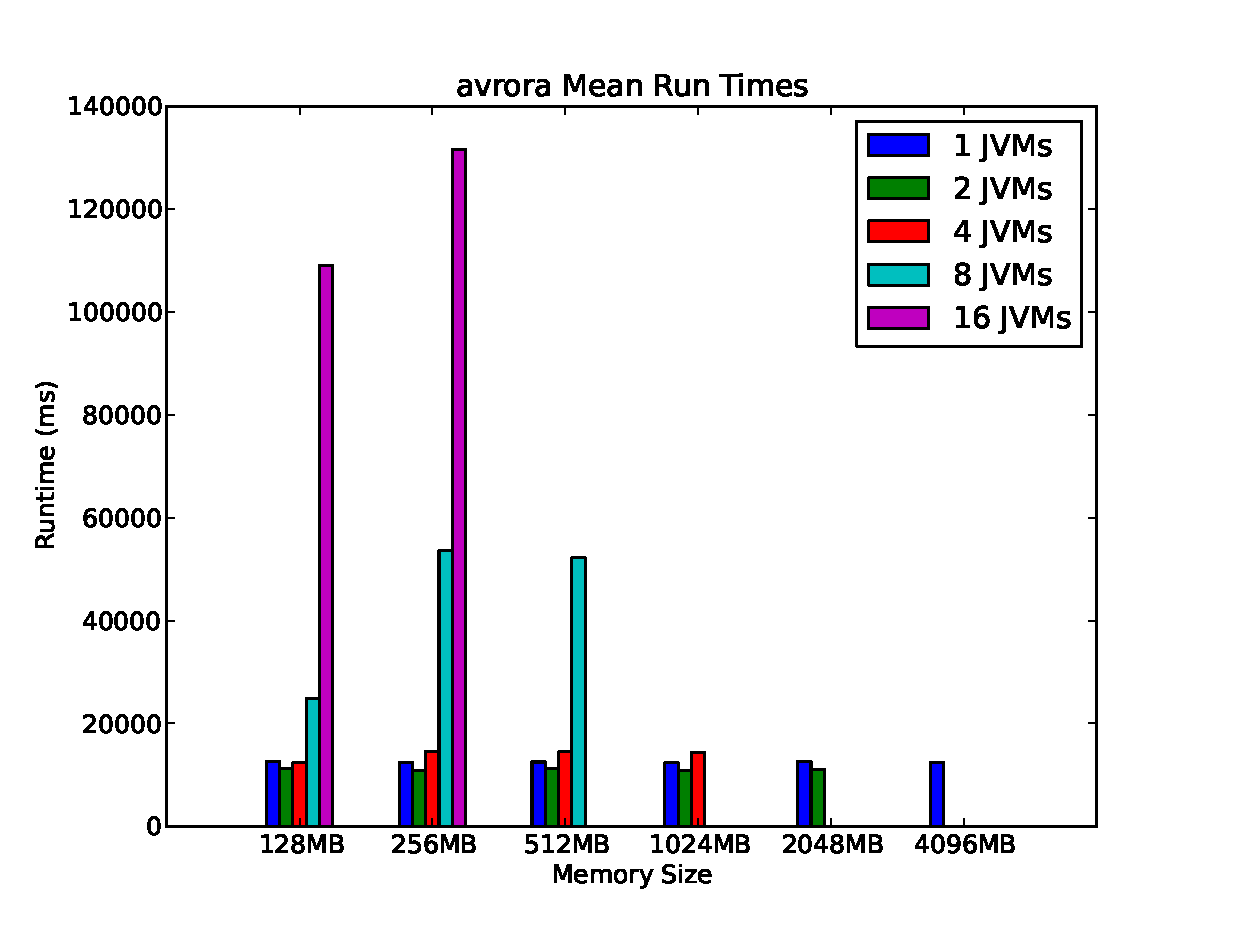
\epsfig{file=figures/avrora.eps, height=2in, width=3in}
\caption{A sample graphic (.eps format)
that has been resized with the \texttt{epsfig} command.}
\end{figure}

%As was the case with tables, you may want a figure
%that spans two columns.  To do this, and still to
%ensure proper ``floating'' placement of tables, use the environment
%\textbf{figure*} to enclose the figure and its caption.
%and don't forget to end the environment with
%{figure*}, not {figure}!

\begin{figure*}
\centering
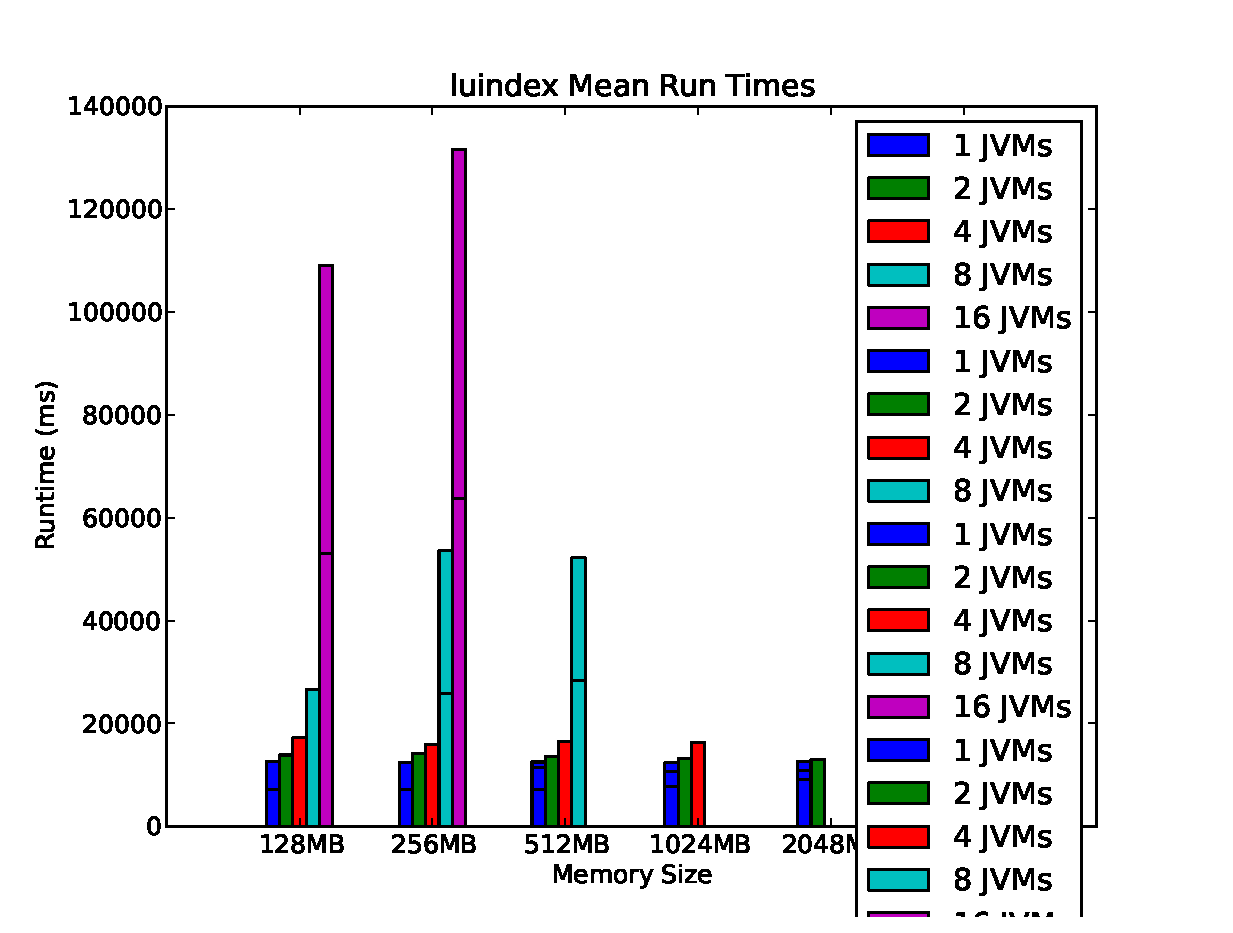
\epsfig{file=figures/luindex.eps}
\caption{A sample black and white graphic (.eps format)
that needs to span two columns of text.}
\end{figure*}

\section{Conclusion}
This paragraph will end the body of this sample document.
Remember that you might still have Acknowledgments or
Appendices; brief samples of these
follow.  There is still the Bibliography to deal with; and
we will make a disclaimer about that here: with the exception
of the reference to the \LaTeX\ book, the citations in
this paper are to articles which have nothing to
do with the present subject and are used as
examples only.
%\end{document}  % This is where a 'short' article might terminate

%ACKNOWLEDGMENTS are optional
\section{Acknowledgments}
Martin
Nathan
Eric

% The following two commands are all you need in the
% initial runs of your .tex file to
% produce the bibliography for the citations in your paper.
\bibliographystyle{abbrv}
\bibliography{JVMTesselation}  % sigproc.bib is the name of the Bibliography in this case
% You must have a proper ".bib" file
%  and remember to run:
% latex bibtex latex latex
% to resolve all references
%
% ACM needs 'a single self-contained file'!
%

\balancecolumns
\end{document}
